\documentclass{article}
\usepackage{graphicx}
\usepackage{hyperref}
\usepackage{amsmath}
\usepackage{amssymb}
\usepackage{enumitem}
\usepackage{float}
\usepackage{textcomp}

\renewcommand\labelitemi{---}

\author{Stephen Lee}
\title{Bitcoin is dead: Long live Bitcoin?}
\date{2018}

\begin{document}
	\maketitle
	
	\section{Introduction}
	In 2008, the Bitcoin white paper was published under the pseudonym Satoshi Nakamoto. The paper combined cryptography with a game theoretic incentive structure to provide secure peer-to-peer financial transactions without needing a trusted 3rd party.  Since then, other projects have modified the Bitcoin rules to create new protocols to handle these transactions. Colloquially referred to as ``cryptocurrencies'', these projects have captured the imagination of many. As of May 3, 2018, the three largest cryptocurrencies by market capitalization are Bitcoin, Ether, and Ripple. This time series analysis looks at those three coins, along with another project, Litecoin, to see if there is any exploitable market inefficiency. Notably, I test for Granger causality and co-integration to see if price movements of one coin can act as an early indicator for another coin. While these results are inconclusive at this point, the appearance of a large ``bubble'' from December 2017 to February 2018 is likely responsible. Preliminary work with the ``post-bubble'' data indicate significant unidirectional causality for each coin, with Bitcoin acting as the most exogenous series. Further, I fit TGARCH models to Bitcoin, Ether, and Ripple and show that investors respond with increased volatility after a negative price shock than for a positive price shock. 
	
	Further work is needed to explain the dramatic rise, and subsequent fall, in price during the two month span from December 2017 to February 2018. In particular, I plan to explore a sentiment analysis approach utilizing Twitter data during those periods. 
	
	\section{Data}
	I gathered transaction-level data on Bitcoin, Ether, Ripple, and Litecoin from the European coin exchange Bitstamp. The raw data includes information about each transaction in the history of the exchange, including the unix-timestamp\footnote{The unix-timestamp is given by the number of seconds that have passed since January 1, 1970 at 12:00:00 am GMT}, trade price, and trade quantity. Several points to consider: 
	\begin{itemize}
		\item The different coins were offered at different points in time. For example, Bitcoin was the first coin offered on the exchange, while Ether was the most recent addition. Thus, for consistency of the analysis I used the earliest date such that trade information exists for each coin. 
		\item Each transaction is marked to the second. In order to use a smooth time series without missing or repeated observations, I found the smallest period of time such that at least one transaction took place for each series. In this case, Litecoin was the limiting factor in calculating the time periods - there was a maximum gap of 5525 seconds between subsequent transactions. Thus, I made a dataset using this as the period length as well as a second dataset that used one-hour as the period length\footnote{Using one hour as the period length created a single missing observation in the Litecoin series.}. Ultimately, for the analysis I used the hourly dataset. 
	\end{itemize}
	
	The final series consisted of hourly periods ranging from Thursday, August 17, 2017 2:00:03 pm to Tuesday, April 24, 2018 4:00:03 am GMT. Figure \ref{allGraphs} show the raw series, and table \ref{desStats} shows the descriptive statistics.

	\begin{figure}[H]
		\centering
		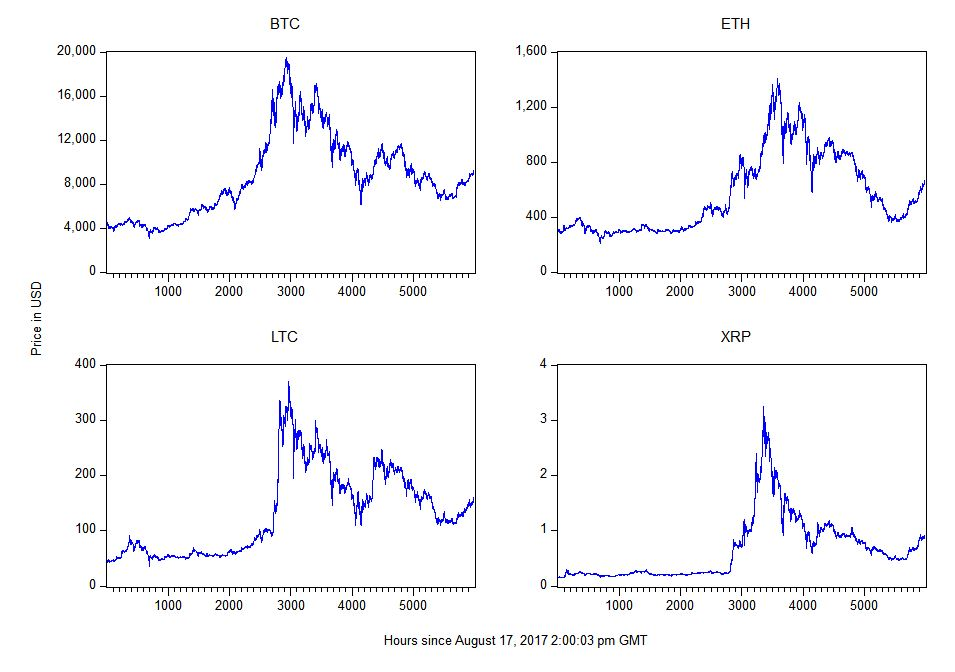
\includegraphics[width = .75\textwidth]{AllCoins_graph.jpg}
		\caption{Time series of each coin in dataset.}
		\label{allGraphs}
	\end{figure}
	
	\begin{table}[H]
		\centering
		\begin{tabular}{|l|r|r|r|r|}
			\hline
			& \multicolumn{1}{l|}{Bitcoin} & \multicolumn{1}{l|}{Ethereum} & \multicolumn{1}{l|}{Ripple} & \multicolumn{1}{l|}{Litecoin} \\ \hline
			Maximum      & \$19537.83                     & \$1405.34                       & \$3.25                    & \$370.28                      \\ \hline
			Minimum      & \$3009.53                      & \$204.85                      & \$0.15                    & \$36.17                      \\ \hline
			Mean         & \$8648.10                      & \$566.08                      & \$0.65                    & \$133.05                      \\ \hline
			St. Dev      & \$3749.17                      & \$284.70                      & \$0.57                    & \$76.66                      \\ \hline
			Observations & 5991                         & 5991                          & 5991                        & 5990                          \\ \hline
		\end{tabular}
		\caption{Descriptive statistics. Prices in USD.}
		\label{desStats}
	\end{table}

	Interestingly, the price for each coin are on different orders of magnitude and include an order of magnitude variation from the minimum to maximum. As the descriptive statistics show in table \ref{desStats}, Bitcoin has a maximum price of \$19,537.83 per BTC and minimum price of \$3009.53 per BTC. On the other end of the spectrum, Ripple has a maximum price of \$3.25 per XRP, and a minimum price of \$0.15 per XRP. Ethereum and Litecoin have similar relative variation. In order to better understand how the series moved in relative terms, I created a normalized series, $\{s^n\}$, by dividing the price at a given point in time by the series mean, $\mu_s$. Mathematically this is to say: 
	\begin{equation}
		s_t^n = \frac{s_t}{\mu_s}
	\end{equation}
	
	Since this helps to normalize the series deviations, we can view this graphically below: 
	\begin{figure}[H]
	\centering
	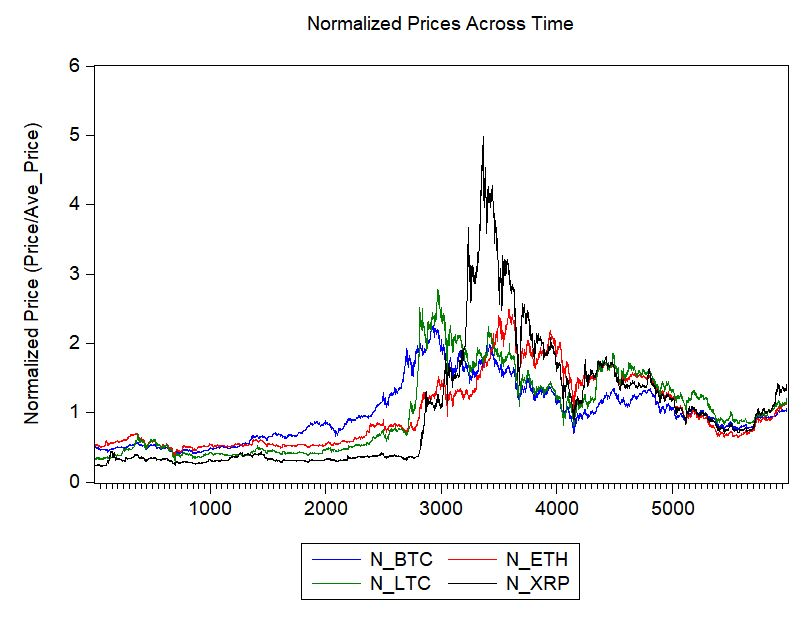
\includegraphics[width = .75\textwidth]{NormalizedPrices_graph.jpg}
	\caption{Overlay of each normalized series in dataset.}
	\end{figure}
	
	While the graph is a bit cluttered, what stands out is that Ripple experienced the largest percent increase at its peak, while Litcoin, Ether, and Bitcoin are all very similar. To get a clearer idea of how the series respond to each other, I restrict the graph to only the two largest coins by market cap - Bitcoin and Ether: 
	\begin{figure}[H]
		\centering
		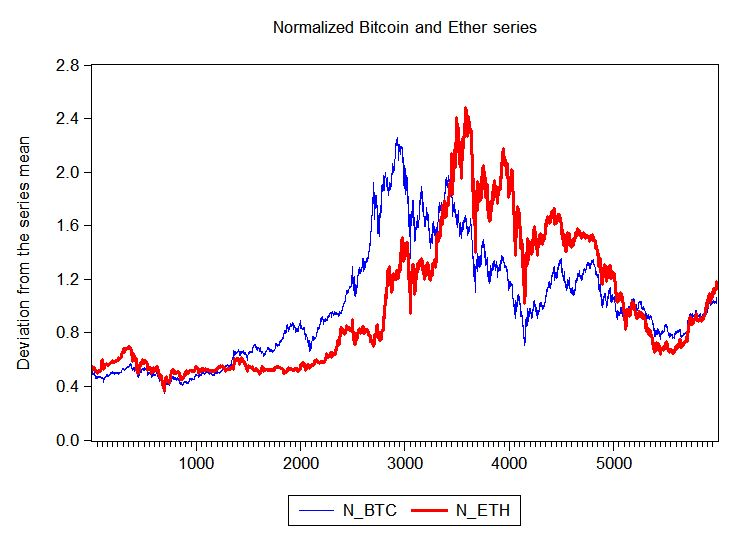
\includegraphics[width = .75\textwidth]{NormalizedPrices_ethBtcGraph.jpg}
		\caption{Overlay of Bitcoin and Ether's normalized series.}
	\end{figure}
	
	Here we see that, in normalized terms, Bitcoin's largest surge and drop seems to occur about a month (i.e. approximately 750 hours) before Ether. Interesting, however, the last month or so in the dataset show much tighter price movements, suggesting a potential change in investor perspective. 
	
	\section{Analysis and Results}
	
	Since the series levels are clearly not stationary, I calculated the series of first differences ($\Delta s_t = s_t - s_{t-1}$) and performed the Augmented Dicky-Fuller test for unit roots. In each differenced series, I am able to reject the null hypothesis that a unit root exists and accept that the level series are all integrated of degree one (i.e. I(1)). Visually we can see these differenced series below:
	
	\begin{figure}[H]
		\centering
		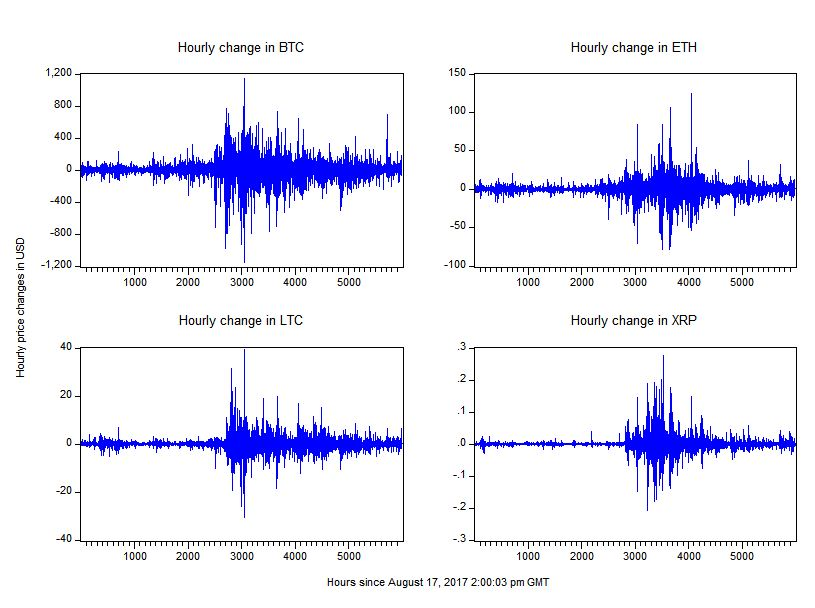
\includegraphics[width = .75\textwidth]{AllCoinsDifferenced_graph.jpg}
		\caption{Time series of each differenced coin series in dataset.}
	\end{figure}
	
	\subsection{Individual Series Analysis}
	While the differenced series do seem to have a time constant mean, the variance is definitely not constant across time. With that in mind, I tested various specifications using ARCH and GARCH errors to see how the data moves. For each series, the ACF and PACF suggest significant autocorrelation for two-periods (i.e. two hours). However, after finding the best-fit ARCH and GARCH, the series of squared residuals still indicates significant autocorrelation and partial autocorrelation. Thus, I finally settled on an AR model with TGARCH errors, suggesting that traders are affected by whether the prices are rising or falling. The results for Bitcoin, Ether, and Ripple are presented below. 
	
	\subsubsection{Bitcoin}
	The best fitting model for the Bitcoin data is an AR(3) with TGARCH error terms. After fitting I find the following model\footnote{Z-statistics in parentheses.}: 
	
	\begin{align}
	\begin{split}
		\Delta BTC_t &= 0.20 \Delta BTC_{t-1} - 0.12 \Delta BTC_{t-2} + 0.03 \Delta BTC_{t-3} + \epsilon_t\\
		 & \quad (15.34) \quad \quad \quad (-8.25) \quad \quad \quad \quad (2.36)
	\end{split}
	\end{align}
	With an error process given by: 
	\begin{align}
	\begin{split}
	E_{t-1}(\epsilon_t^2)  &= 23.25 + 0.068 \epsilon^2_{t-1} + 0.02 D_{t-1} \epsilon^2_{t-1} + 0.926 h_{t-1}\\
	& \quad (14.23) \quad (23.13) \quad \quad (3.82) \quad \quad \quad \quad (530.00)
	\end{split}
	\end{align}
	
	Next we look at the ACF and PACF of the residual and squared residual series from this estimation. We find that they mirror a white noise process.  
	\begin{figure}[H]
		\centering
		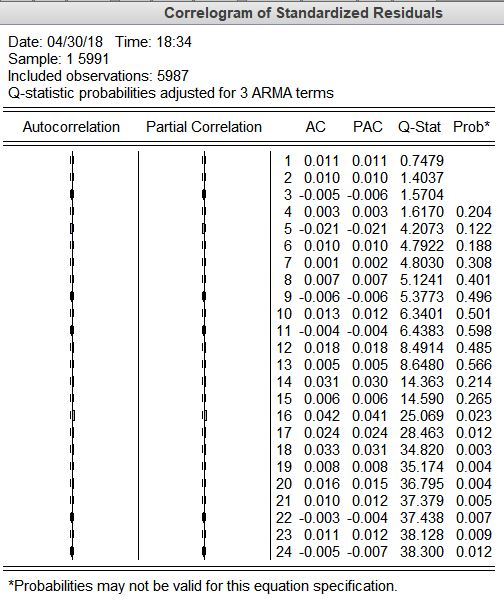
\includegraphics[width = .75\textwidth]{btcTGARCH_residCor.jpg}
		\caption{ACF and PACF of the residuals from the above AR(2) model with TGARCH errors on the differenced Bitcoin series.}
	\end{figure}

	\begin{figure}[H]
		\centering
		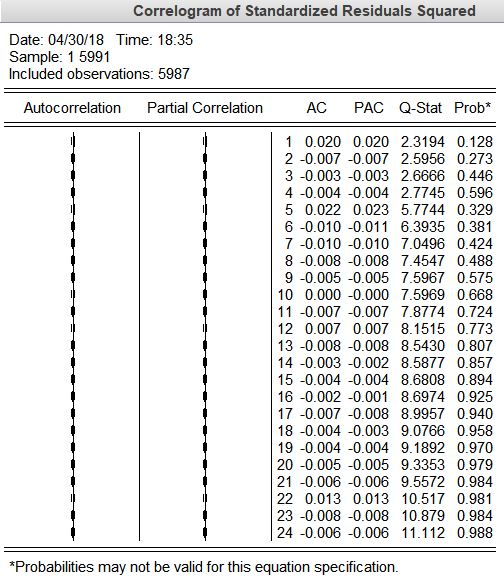
\includegraphics[width = .75\textwidth]{btcTGARCH_residSqCor.jpg}
		\caption{ACF and PACF of the squared residuals from AR(2) model with TGARCH errors on the differenced Bitcoin series.}
	\end{figure}

	\subsubsection{Ether}
	
	The best fitting model for the Ether data is an AR(2) with TGARCH error terms. After fitting I find the following model\footnote{Z-statistics in parentheses.}: 
	
	\begin{align}
	\begin{split}
	\Delta ETH_t &= 0.15 \Delta ETH_{t-1} - 0.10 \Delta ETH_{t-2} + \epsilon_t\\
	& \quad (12.02) \quad \quad \quad \quad (-6.71) 
	\end{split}
	\end{align}
	
	With an error process given by: 
	\begin{align}
	\begin{split}
	E_{t-1}(\epsilon_t^2)  &= 0.12 + 0.11 \epsilon^2_{t-1} + 0.02 D_{t-1} \epsilon^2_{t-1} + 0.89 h_{t-1}\\
	& \quad (12.72) \,\, (21.36) \quad \quad (2.84) \quad \quad \quad \quad (270.10)
	\end{split}
	\end{align}
	
	We again look at the ACF and PACF of the residual and squared residual series from this estimation and confirm that they mirror a white noise process. 
	
	\begin{figure}[H]
		\centering
		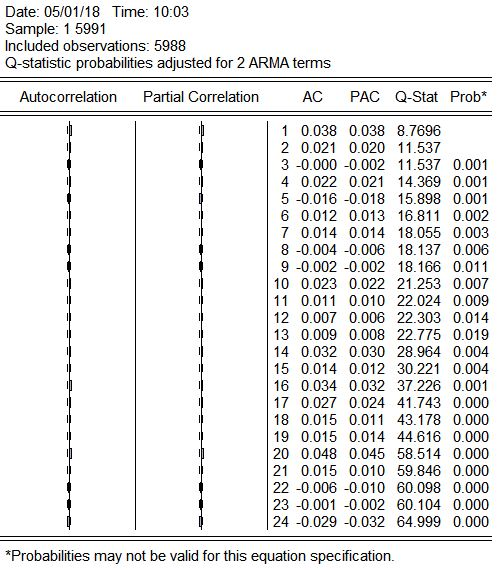
\includegraphics[width = .75\textwidth]{ethTGARCH_residCor.jpg}
		\caption{ACF and PACF of the residuals from the above AR(2) model with TGARCH errors on the differenced Ether series.}
	\end{figure}
	
	\begin{figure}[H]
		\centering
		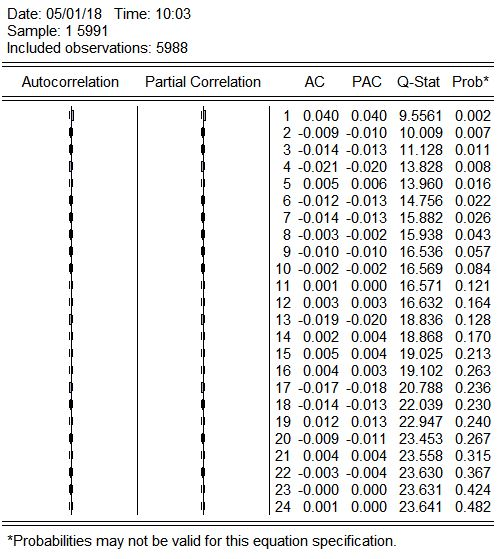
\includegraphics[width = .75\textwidth]{ethTGARCH_residSqCor.jpg}
		\caption{ACF and PACF of the squared residuals from AR(2) model with TGARCH errors on the differenced Ether series.}
	\end{figure}
	
	\subsubsection{Ripple}
	
	The best fitting model for the Ether data is an AR(2) with TGARCH error terms. After fitting I find the following model\footnote{Z-statistics in parentheses.}: 
	
	\begin{align}
	\begin{split}
	\Delta XRP_t &= 0.13 \Delta XRP_{t-1} - 0.10 \Delta XRP_{t-2} + \epsilon_t\\
	& \quad (9.67) \quad \quad \quad \quad (-6.68) 
	\end{split}
	\end{align}
	
	With an error process given by: 
	\begin{align}
	\begin{split}
	E_{t-1}(\epsilon_t^2)  &= 0.000000312 + 0.14 \epsilon^2_{t-1} + 0.014 D_{t-1} \epsilon^2_{t-1} + 0.87 h_{t-1}\\
	& \quad (35.14) \quad \quad \quad \quad (26.60) \quad \quad (1.97) \quad \quad \quad \quad (261.57)
	\end{split}
	\end{align}
	
	We again look at the ACF and PACF of the residual and squared residual series from this estimation and confirm that they mirror a white noise process. 
	
	\begin{figure}[H]
		\centering
		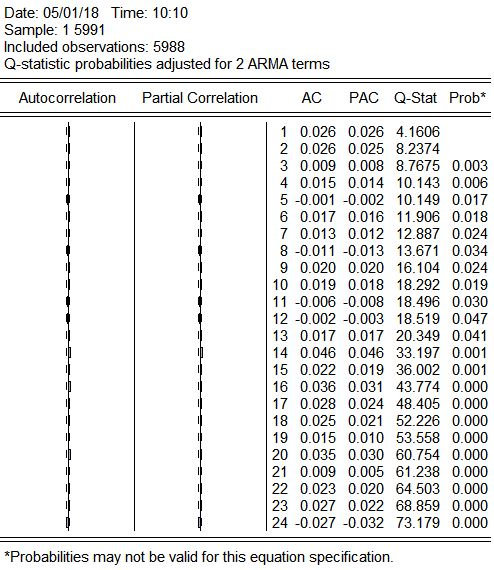
\includegraphics[width = .75\textwidth]{xrpTGARCH_residCor.jpg}
		\caption{ACF and PACF of the residuals from the above AR(2) model with TGARCH errors on the differenced Ripple series.}
	\end{figure}
	
	\begin{figure}[H]
		\centering
		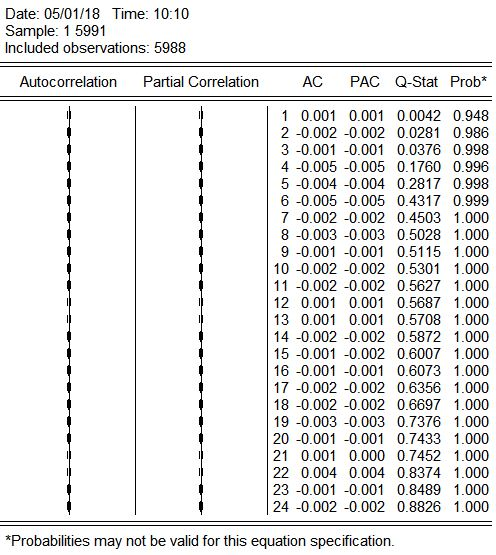
\includegraphics[width = .75\textwidth]{xrpTGARCH_residSqCor.jpg}
		\caption{ACF and PACF of the squared residuals from AR(2) model with TGARCH errors on the differenced Ripple series.}
	\end{figure}
	 
	\subsection{Cointegrated Series Analysis}
	After finding a model for Bitcoin, Ether, and Ripple that only rely on their own history, next, I test for Granger causality in the level-series\footnote{The lag length for the level series was determined by optimizing the AIC in a standard VAR.} to determine if information of the other coins can improve estimates for a given coin. I find significant bi-directional causality in most of the major coin pairs. The only notable unidirectional exception is Bitcoin causing Litecoin. We see the results below: 
	
	\begin{figure}[H]
		\centering
		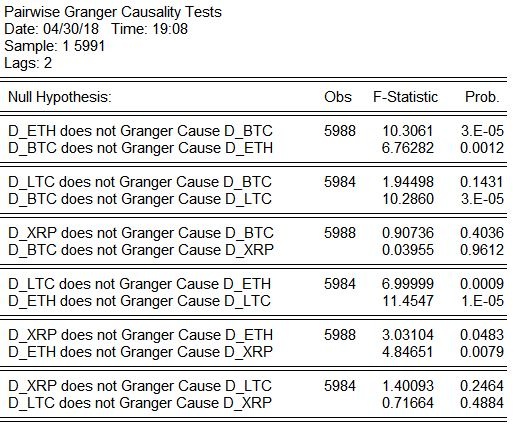
\includegraphics[width = .75\textwidth]{GrangerCausality_levels.jpg}
		\caption{Granger causality tests using the stationary differenced series.}
	\end{figure}
	
	Note, however, that these results are for the entire series. Restricting the sample to ``post-bubble'' data results in significant unidirectional Granger causality for each coin, with Bitcoin acting as the first mover. 
	
	Next we look for co-integrating equations using the Johansen system test with two lags as described above. The results from both the trace and maximum eigenvalue statistics indicate three co-integrating equations at the 5\% level. To further motivate and understand the possibility of co-integration, we can look at the relative prices of each series. Specifically, I calculate the price of a given coin as denominated in another coin. For example, the Bitcoin and Ether pair would tell us how many Bitcoin it costs to buy a single Ether across our sample. The idea is to check if there exists a relatively consistent relationship between the coins. A graph of each pair is presented below:
	
	\begin{figure}[H]
	 	\centering
	 	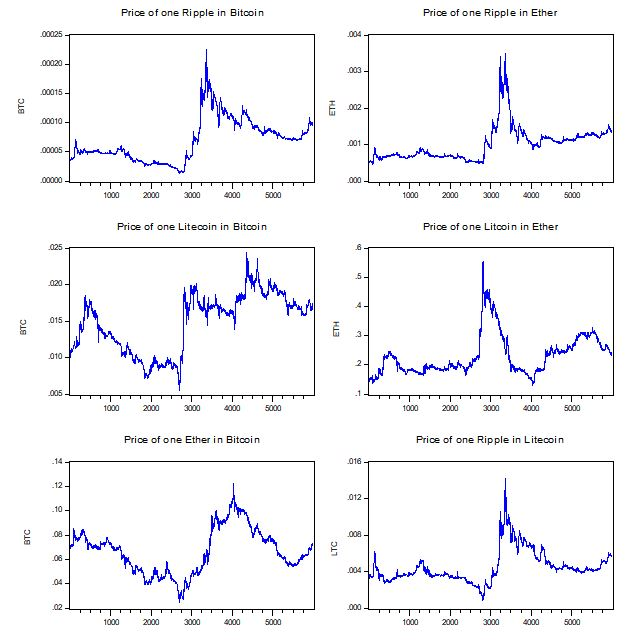
\includegraphics[width = .75\textwidth]{RelativePrices_allCoins.jpg}
	 	\caption{The relative price for each coin pair.}
	\end{figure}

	These graphs, while undoubtedly noisy, tell the story of different relative price jumps, but also of a potential correction to a long-run relationship. Specifically, we see that each coin was ``cheap'' to buy with Bitcoin up until about the 2750th hour in the dataset (this corresponds to approximately December 10, 2017). At this point, Litecoin, Ripple, and Ether all began to increase in price (and in that respective order) relative to Bitcoin. The order of the price increases are exemplified in the graphs on the right-hand-side, which show that Ripple and Litecoin both became relatively ``expensive'' to buy with Ether, before returning to the previous level. This is to say that first, the price of Litecoin increased away from the long-run equilibrium. This was followed by a more dramatic increase in the price of Ripple, and finally a slower, but substantial, increase in the price of Ether. Finally we see that, through some mechanism, the prices correct back to what appears to be an average ratio between the pairs. Thus, while volatile indeed, there does appear to be the possibility of persistent long-run relationships.
	
	With that said, I run the vector error correction model with three co-integrating equations, and no trend or intercept, as suggested by the Johansen system test. The results are presented in Figure \ref{VEC} below: 
	
	\begin{figure}[H]
		\centering
		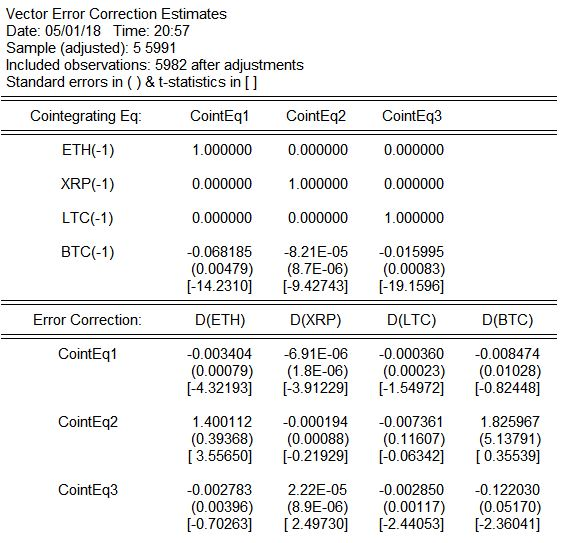
\includegraphics[width = .75\textwidth]{VEC_Results.jpg}
		\caption{Vector Error Correction model with three co-integrating equations and no time-trend or intercept. }
		\label{VEC}
	\end{figure}

	While this table will take me some time to understand and explain in detail, the parts that stand out is the non-zero speed of adjustment for both Litecoin and Bitcoin in cointegrating equation 3. Besides that, nothing stands out as statistically and economically significant. Based on the graphs above, the next steps are to explore longer lag lengths, or by using a restricted dataset.  
	
	\section{Conclusion}
	A preliminary analysis of Bitcoin, Ether, Ripple, and Litecoin suggest the following: 
	\begin{itemize}
		\item \textbf{An apparent bubble began for each coin starting around December 2017 until early February 2018.} Figure 2 shows the ratio of each coin's price to it's series mean. We see that Ripple (XRP) experienced the most dramatic price increase during the bubble with prices of nearly 5 times the average price. In contrast, Bitcoin, Ether, and Litecoin all saw a maximum price of about 2.5 times their mean price during this period. 
		\item \textbf{The maximum price of each coin occurred at different points in time, possibly indicating causality with a lag length of a couple weeks during the bubble period.} Specifically, Bitcoin was the first to reach it's maximum, followed closely by Litecoin, then Ripple, and finally Ether. This tells us that Bitcoin is likely the most exogenous coin, with the others following it's movement at various lag lengths. If, however, we restrict the dataset to the ``post-bubble'' period, we find significant uni-directional granger causality indicating that Bitcoin is the first mover with all other coin's following it's movement 2 hours later.   
		\item \textbf{We cannot reject the possibility of a long-run relationship between coin pairs.} Based on the exchange rates in Figure 12, there was a dramatic change in the exchange rates from early December 2017 to early February 2018. However, after this apparent bubble, the exchange rates have all returned to levels that are consistent with ``pre-bubble'' rates. More analysis and data are needed to confidently investigate co-integration. 
	\end{itemize} 

	\subsubsection{Further Research}
	The next steps in this analysis are to compare various subsamples of this data set. Specifically, I will test whether the ``pre-bubble'' and ``post-bubble'' series have similar behavior, or if the ``bubble mainia'' changed investor perspective. Further research is also needed to explain the ``bubble'' that started in late-November/early-December 2017 and ended in late-January/early-February 2018. For that, I intend to perform a sentiment analysis using Twitter data to see if quantity of positive and negative tweets correlate with large price changes.  
	
\end{document}

% Itemize
\begin{itemize}
	\item
\end{itemize}

% enumerate
\begin{enumerate}
	\item
\end{enumerate}

% Figures
\begin{figure}[H]
	\centering
	\includegraphics[width = .75\textwidth]{}
	\caption{}
\end{figure}

% Equations
\begin{align}
\begin{split}
\end{split}
\end{align}

% Paragraph
\begin{flushleft}
\end{flushleft}

% Fancy 
\begin{equation}
\mathcal{L}(T,B,\lambda) = 
\end{equation}

% Partials
\begin{align}
\frac{\partial \mathcal{L}}{\partial T} &= 
\frac{\partial \mathcal{L}}{\partial B} &= 
\frac{\partial \mathcal{L}}{\partial \lambda} &= 
\end{align}

%Piecewise
\begin{displaymath}
function = \left\{
\begin{array}{lr}
0 & \quad P\textsubscript{C} < P\textsubscript{P}\\
U\textsubscript{0} & \quad  P\textsubscript{C} > P\textsubscript{P}
\end{array}
\right.
\end{displaymath}
